\documentclass{beamer}
\usepackage[utf8]{inputenc}
\usetheme{Madrid}
\usepackage{graphicx}
\usepackage{amssymb}


%Information to be included in the title page:
\title[Sierpinski Gasket]{The Cantor Set and the Sierpinski Gasket}
\subtitle{DRP Presentation}
\author{Andrew Gao}

\date{December 2018}
 
 
 
\begin{document}
\frame{\titlepage}
 
\begin{frame}
\frametitle{Textbook}
\begin{center}
The textbook I used was \textit{Measure, Topology, and Fractal Geometry} 2\textsuperscript{nd} Edition by Gerald Edgar.\\ \vspace{2em}
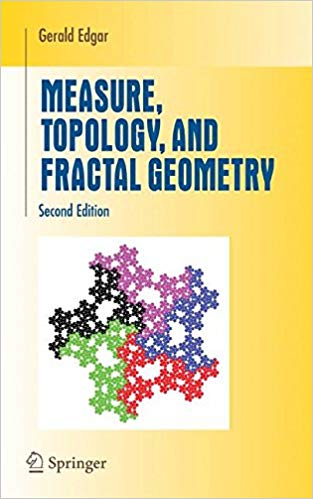
\includegraphics[scale=0.25]{mtfg.jpg}
\end{center}
\end{frame}
 
\begin{frame}{The Cantor Set}
\begin{center}
We define the Cantor Set $C = \bigcap_{k\in\mathbb{N}}C_{k}$,\\ with each $C_k$ being constructed by tremas as seen below\\ \vspace{2em}
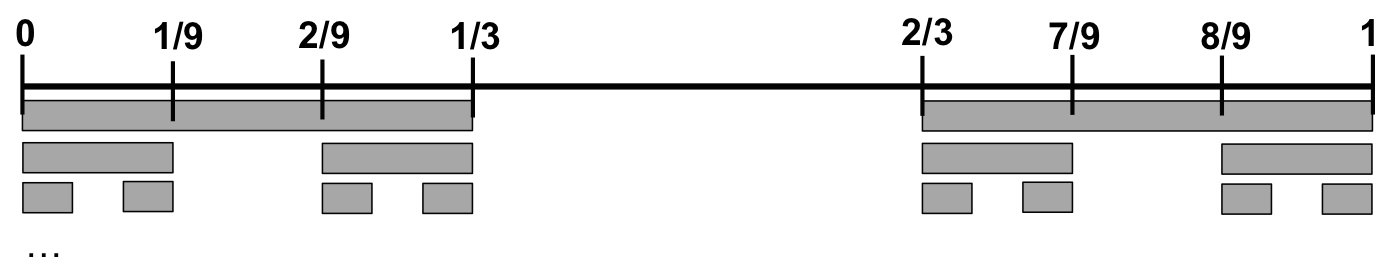
\includegraphics[scale=0.4]{canto1.png}
\end{center}
\end{frame}

\begin{frame}{Properties of the Cantor Set}
\begin{center}
We see that each set $C_k$ consists of $2^k$ intervals, each of length $(\frac{1}{3})^k$\\ \vspace{1em}
Traditionally, we would define the \textbf{total length} of each $C_k$ as $$\lim_{k\to\infty} (\frac{2}{3})^k$$
\end{center}
\end{frame}

\begin{frame}{A Unique Parallel between the Set and Ternary Decimals}
\begin{center}
\textbf{Proposition}: Any $x \in [0,1]$ belongs to the Cantor Set if and only if $x$ has a base 3 expansion using only digits 0 and 2.
\end{center}
\end{frame}

\begin{frame}{The Sierpinski Gasket}
\begin{center}
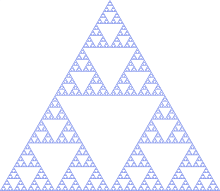
\includegraphics[scale=.5]{triangle.png} \hspace{2em}
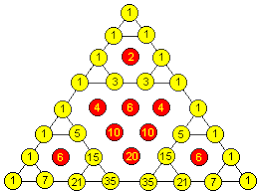
\includegraphics[scale=0.5]{pascal.png}
\end{center}
\end{frame}

\begin{frame}{The Sierpinski Gasket}
\begin{center}Here is an example of a construction by tremas.\\ \vspace{2em}\end{center}
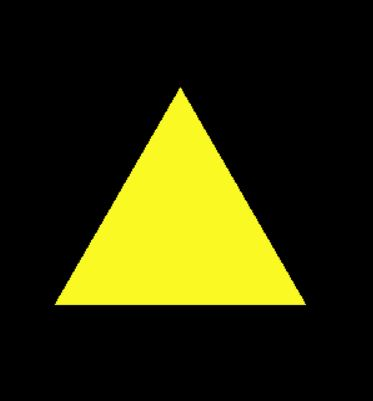
\includegraphics[scale=.25]{gasket0.JPG} \hspace{1em}
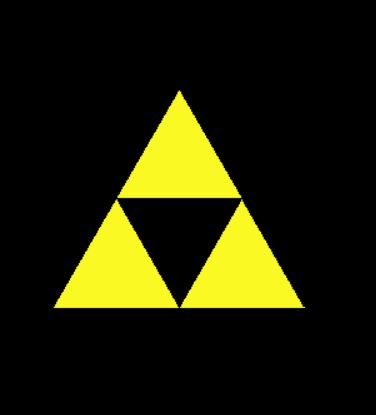
\includegraphics[scale=.25]{gasket1.JPG} \hspace{1em}
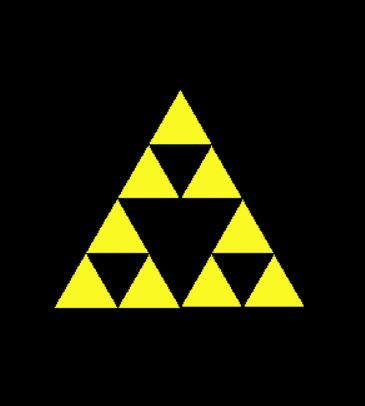
\includegraphics[scale=.25]{gasket2.JPG} \hspace{1em}
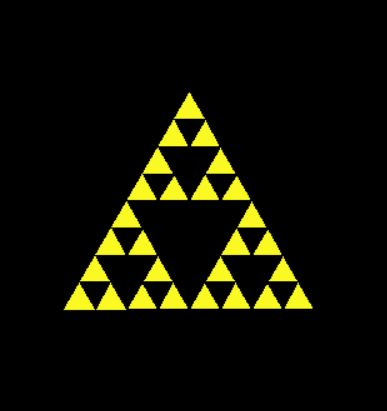
\includegraphics[scale=.25]{gasket3.JPG} \hspace{1em}
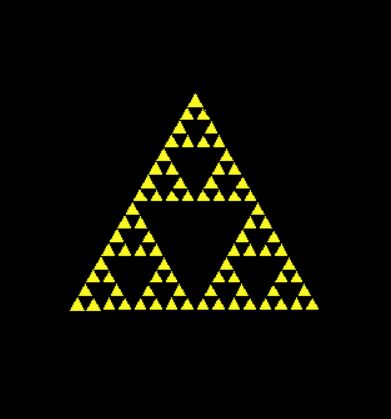
\includegraphics[scale=.25]{gasket4.JPG} 
\end{frame}

\begin{frame}{Properties of the Gasket}
We define $S =\bigcap_{k\in\mathbb{N}}S_{k}$\\ \vspace{1em}
Every $S_{k}$ has $3^k$ triangles, each of which has side length $2^{-k}$.\\ \vspace{2em}
Traditionally: the \textbf{total area} of $S$ is $3^k \cdot \frac{\sqrt{3}}{4} \cdot (2^{-k})^2$. \\ \vspace{1em}
Traditionally: the \textbf{total length} of $S$ is $3^k \cdot 3 \cdot 2^{-k}$. \\
\end{frame}

\begin{frame}{Topological Dimension}
How would we intuitively create this idea of the dimension of a set?
\end{frame}

\begin{frame}{Topological Dimension of the Cantor Set}
\textbf{Definitions:} \\

Let $S$ be a metric space and let $\mathcal{A}$ be an open cover of $S$.\\ \vspace{1em}A \textbf{\emph{refinement}} of $\mathcal{A}$ is an open cover $\mathcal{B}$ of $S$ such that for every $B \in \mathcal{B}$, there exists an $A\in\mathcal{A}$ where $B\subseteq A$.\\ \vspace{1em}

We define a space $S$ to be \textbf{zero-dimensional} if every finite \textbf{open cover} for $S$ has a finite \textbf{refinement} that is a \textbf{clopen partition}.
\end{frame}

\begin{frame}
\begin{center}
\Huge{Thanks for listening!}
\end{center}
\end{frame}
\end{document}